\documentclass[a4paper,11pt]{article}

% ============================================================
%  Le Collé — Séance 1 : Déterminants, courbes paramétrées
%  © 2026 Ahmed Amine Ouqlani
% ============================================================

% ---------- Polices ----------
\usepackage[utf8]{inputenc}
\usepackage[T1]{fontenc}
\usepackage[sc]{mathpazo}          % texte et mathématiques : Palatino
\usepackage[scaled=0.88]{helvet}   % titres et repères : linéale
\linespread{1.07}
\usepackage{amsmath,amssymb,amsthm,mathrsfs,stmaryrd}
\usepackage{microtype}

% ---------- Mise en page ----------
\usepackage[a4paper,top=2.3cm,bottom=2.3cm,left=2.4cm,right=2.4cm,
            headheight=14pt,headsep=0.8cm,footskip=1.1cm]{geometry}
\setlength{\parindent}{0pt}
\setlength{\parskip}{0.45em plus 0.15em minus 0.1em}
\raggedbottom
\emergencystretch=1.5em
\clubpenalty=10000 \widowpenalty=10000 \displaywidowpenalty=10000 \brokenpenalty=10000

% ---------- Couleurs : un bleu de nuit, un ocre, des gris ----------
\usepackage{xcolor}
\definecolor{Ink}{HTML}{1C2533}
\definecolor{Bleu}{HTML}{1F3A5F}
\definecolor{BleuMoyen}{HTML}{4A6A8F}
\definecolor{BleuClair}{HTML}{9DB2C9}
\definecolor{Fond}{HTML}{F2F4F7}
\definecolor{Ocre}{HTML}{B07A26}
\definecolor{Brique}{HTML}{A23B2A}
\definecolor{Gris}{HTML}{5E6672}
\definecolor{Filet}{HTML}{C5CCD6}

% ---------- Packages ----------
\usepackage{enumitem}
\setlist{itemsep=0.25em,topsep=0.35em,parsep=0pt}
\setlist[itemize]{label=\textcolor{BleuMoyen}{\small\textbullet},leftmargin=1.4em}
\setlist[enumerate]{leftmargin=1.8em,label=\textsf{\small\color{Bleu}\arabic*.}}
\usepackage{booktabs,array,multicol}
\usepackage{needspace,float}
\usepackage[font=small,labelfont={sf,color=Bleu},labelsep=period,skip=6pt]{caption}
\usepackage{tikz}
\usetikzlibrary{arrows.meta,calc,decorations.markings}
\usepackage{pgfplots}
\pgfplotsset{compat=1.17}
\usepackage{tkz-tab}
\usepackage[most]{tcolorbox}
\usepackage{titlesec,titletoc}
\usepackage{fancyhdr,lastpage,etoolbox}
\usepackage[colorlinks=true,linkcolor=Bleu,urlcolor=Bleu,citecolor=Bleu,
            pdftitle={Le Collé — TD Courbes paramétrées (énoncés)},pdfauthor={Ahmed Amine Ouqlani}]{hyperref}

\numberwithin{equation}{section}
\numberwithin{figure}{section}
\numberwithin{table}{section}

% ---------- Titres ----------
% Chapitres (sections) : grand numéro, titre en linéale, filet ocre
\titleformat{\section}[display]
  {\normalfont\sffamily\color{Ink}}
  {{\small\color{Gris}\textls[200]{\MakeUppercase{Chapitre}}}\\[-0.2em]%
   {\fontsize{64}{64}\selectfont\color{BleuClair}\thesection}}
  {0.4em}
  {\fontsize{25}{30}\selectfont\bfseries}
  [\vspace{0.5em}{\color{Ocre}\rule{3.2cm}{1.4pt}}]
\titlespacing*{\section}{0pt}{0pt}{1.6em}
\titleformat{name=\section,numberless}[display]
  {\normalfont\sffamily\color{Ink}}{}{0pt}{\fontsize{25}{30}\selectfont\bfseries}
  [\vspace{0.5em}{\color{Ocre}\rule{3.2cm}{1.4pt}}]
\titlespacing*{name=\section,numberless}{0pt}{0pt}{1.6em}

\titleformat{\subsection}
  {\needspace{5\baselineskip}\normalfont\sffamily\Large\bfseries\color{Ink}}
  {\color{Bleu}\thesubsection}{0.8em}{}
\titlespacing*{\subsection}{0pt}{1.8em}{0.5em}
\titleformat{\subsubsection}
  {\needspace{5\baselineskip}\normalfont\sffamily\large\bfseries\color{Ink}}
  {\color{Bleu}\thesubsubsection}{0.7em}{}
\titlespacing*{\subsubsection}{0pt}{1.6em}{0.4em}
\titleformat{\paragraph}[runin]{\normalfont\sffamily\bfseries\color{Ink}}{}{0pt}{}[.]
\titlespacing*{\paragraph}{0pt}{0.9em}{0.6em}
\setcounter{secnumdepth}{3}
\setcounter{tocdepth}{2}

% ---------- Table des matières ----------
\titlecontents{section}[0pt]{\addvspace{0.7em}\sffamily\bfseries\color{Ink}}
  {\makebox[2.2em][l]{\color{Bleu}\thecontentslabel}}{}{\hfill\contentspage}[\addvspace{0.2em}]
\titlecontents{subsection}[2.2em]{\small\linespread{1}\selectfont}
  {\makebox[2.6em][l]{\color{Gris}\thecontentslabel}}{}{\titlerule*[0.7pc]{.}\contentspage}

% ---------- En-têtes et pieds de page ----------
\pagestyle{fancy}
\fancyhf{}
\renewcommand{\sectionmark}[1]{\markboth{\thesection\quad#1}{}}
\fancyhead[L]{\footnotesize\sffamily\color{Gris}\leftmark}
\fancyhead[R]{\footnotesize\sffamily\scshape\color{Gris}Le Collé}
\fancyfoot[C]{\small\sffamily\color{Ink}\thepage}
\fancyfoot[L]{\scriptsize\sffamily\hyperlink{toc}{\color{Filet}sommaire}}
\renewcommand{\headrulewidth}{0.4pt}
\renewcommand{\headrule}{{\color{Filet}\hrule height\headrulewidth width\headwidth}}
\renewcommand{\footrulewidth}{0pt}
\fancypagestyle{plain}{\fancyhf{}\fancyfoot[C]{\small\sffamily\color{Ink}\thepage}\renewcommand{\headrulewidth}{0pt}}

% ---------- Énoncés ----------
\newtheoremstyle{enonce}{0pt}{0pt}{}{}{\sffamily\bfseries\color{Bleu}}{.}{0.5em}
  {\thmname{#1}\thmnumber{~#2}\thmnote{\ \normalfont\sffamily\color{Ink}(#3)}}
\newtheoremstyle{exemple}{0.9em}{0.9em}{}{}{\sffamily\bfseries\color{BleuMoyen}}{.}{0.5em}
  {\thmname{#1}\thmnumber{~#2}\thmnote{\ \normalfont\sffamily\color{Ink}(#3)}}
\newtheoremstyle{remarque}{0.7em}{0.7em}{}{}{\sffamily\itshape}{.}{0.5em}{\thmname{#1}\thmnote{\ (#3)}}
\theoremstyle{enonce}
\newtheorem{definition}{Définition}[section]
\newtheorem{theoreme}[definition]{Théorème}
\newtheorem{proposition}[definition]{Proposition}
\newtheorem{corollaire}[definition]{Corollaire}
\theoremstyle{exemple}
\newtheorem{exemple}[definition]{Exemple}
\theoremstyle{remarque}
\newtheorem*{remarque}{Remarque}

\tcbset{
  defi/.style={enhanced,breakable,colback=white,colframe=white,boxrule=0pt,arc=0pt,
     borderline west={1.2pt}{0pt}{Bleu},left=11pt,right=4pt,top=3pt,bottom=3pt,
     before skip=1.1em,after skip=1.1em},
  thm/.style={enhanced,breakable,colback=Fond,colframe=Fond,boxrule=0pt,arc=0pt,
     borderline west={2.4pt}{0pt}{Bleu},left=11pt,right=8pt,top=6pt,bottom=6pt,
     before skip=1.2em,after skip=1.2em}}
\tcolorboxenvironment{definition}{defi}
\tcolorboxenvironment{theoreme}{thm}
\tcolorboxenvironment{proposition}{thm}
\tcolorboxenvironment{corollaire}{thm}

\renewcommand{\proofname}{Démonstration}
\renewcommand{\qedsymbol}{\textcolor{BleuClair}{$\blacksquare$}}
\makeatletter
\renewenvironment{proof}[1][\proofname]{\par\pushQED{\qed}\normalfont
  \topsep0.5em\relax\trivlist\item[\hskip\labelsep\sffamily\itshape\color{Gris}#1.]\ignorespaces}
  {\popQED\endtrivlist\@endpefalse}
\makeatother

% ---------- Méthode : filets haut et bas, titre en bandeau ----------
\makeatletter\newcommand{\methlabelfix}{\protected@edef\@currentlabel{\thetcbcounter}}\makeatother
\newtcolorbox[auto counter,number within=section]{methode}[2][]{%
  enhanced,unbreakable,colback=white,colframe=white,boxrule=0pt,arc=0pt,
  borderline north={0.9pt}{0pt}{Bleu},borderline south={0.9pt}{0pt}{Bleu},
  left=4pt,right=4pt,top=8pt,bottom=8pt,before skip=1.4em,after skip=1.4em,
  before upper={\methlabelfix\phantomsection\addcontentsline{met}{metentry}{\protect\makebox[2.6em][l]{\thetcbcounter}#2}%
     {\sffamily\bfseries\small\color{white}\colorbox{Bleu}{\strut\ MÉTHODE~\thetcbcounter\ }}%
     \ \ {\sffamily\bfseries\color{Bleu}#2}\par\smallskip},#1}

% ---------- Repères pédagogiques : un filet de couleur, un mot-clé ----------
\newcommand{\definirbloc}[3]{% nom, couleur, libellé
  \newtcolorbox{#1}[1][]{enhanced,breakable,blanker,
    borderline west={1.4pt}{0pt}{#2},left=10pt,right=2pt,top=1pt,bottom=1pt,
    before skip=1em,after skip=1em,
    before upper={{\sffamily\bfseries\footnotesize\color{#2}\textls[120]{\MakeUppercase{#3}}}\quad},##1}}
\definirbloc{reflexe}{Bleu}{Réflexe}
\definirbloc{astuce}{Ocre}{Astuce}
\definirbloc{attention}{Brique}{Attention}
\definirbloc{enpratique}{BleuMoyen}{En pratique}
\definirbloc{plusloin}{Gris}{Pour aller plus loin}
\definirbloc{strategie}{Bleu}{Stratégie}
\definirbloc{lecture}{BleuMoyen}{Lire le schéma}
% compatibilité avec les parties reprises
\newenvironment{garde}{\begin{attention}}{\end{attention}}
\newenvironment{complementHP}{\begin{plusloin}}{\end{plusloin}}
\newenvironment{interpretation}{\begin{enpratique}}{\end{enpratique}}

% ---------- Exercices, corrigés ----------
\newcounter{exo}[section]
\renewcommand{\theexo}{\thesection.\arabic{exo}}
\newcommand{\niveau}[1]{{\color{Ocre}\footnotesize
  \ifcase#1\or$\bullet\circ\circ\circ\circ$\or$\bullet\bullet\circ\circ\circ$\or$\bullet\bullet\bullet\circ\circ$%
  \or$\bullet\bullet\bullet\bullet\circ$\or$\bullet\bullet\bullet\bullet\bullet$\fi}}
\newcommand{\serie}[1]{\par\needspace{8\baselineskip}\vspace{1.5em}%
  \noindent{\sffamily\bfseries\color{Bleu}#1}\par\nobreak\vspace{-0.4em}%
  \noindent{\color{Filet}\rule{\linewidth}{0.4pt}}\par\nobreak\vspace{0.1em}}
\newenvironment{exo}[3]{%
  \par\needspace{5\baselineskip}\vspace{0.75em}\refstepcounter{exo}\label{e:#1}%
  \def\exolab{#1}%
  \noindent{\sffamily\bfseries\color{Bleu}Exercice~\theexo}\quad\niveau{#2}%
  \hfill{\footnotesize\sffamily\color{Gris}#3}\par\nobreak\vspace{0.15em}}%
  {\par\nopagebreak\noindent\hfill{\scriptsize\sffamily\hyperref[c:\exolab]{\color{Gris}corrigé p.~\pageref{c:\exolab}}}\par}
\newenvironment{corrige}[1]{%
  \par\needspace{6\baselineskip}\vspace{1em}\phantomsection\label{c:#1}%
  \noindent{\sffamily\bfseries\color{Bleu}Exercice~\ref{e:#1}}\quad
  {\scriptsize\sffamily\hyperref[e:#1]{\color{Gris}énoncé p.~\pageref{e:#1}}}\par\nobreak\vspace{0.2em}}%
  {\hfill\textcolor{BleuClair}{$\square$}\par}
\newcommand{\etape}[1]{\par\smallskip\noindent{\sffamily\bfseries\small\color{BleuMoyen}#1.}\ }
\newenvironment{solution}{\par\noindent{\sffamily\bfseries\small\color{BleuMoyen}Solution.}\ }{\hfill\textcolor{BleuClair}{$\square$}\par}
\newcommand{\chercher}{\par\smallskip\noindent{\color{Filet}\rule[0.5ex]{1.2cm}{0.4pt}}\
  {\footnotesize\sffamily\itshape\color{Gris}laisser chercher l'étudiant avant de poursuivre}\par\smallskip}

% ---------- Guide de séance ----------

\newcommand{\marge}[1]{\leavevmode\marginpar{\raggedleft\scriptsize\sffamily\color{Gris}\textls[100]{\MakeUppercase{#1}}}\ignorespaces}
\newcommand{\Etape}[4]{%
  \subsection[Étape #1 --- #3 {\color{Gris}(#2)}]{#3}\label{etape:#1}%
  \noindent{\small\sffamily\color{Gris}{\color{Ocre}\bfseries Étape #1}\quad·\quad #2\quad·\quad #4}\par\medskip}
\newcommand{\question}[1]{\par\smallskip\noindent{\sffamily\bfseries\small\color{BleuMoyen}Question.}\ \textit{#1}\par\smallskip}
\newcommand{\rappel}[1]{\par\smallskip\noindent\phantomsection\addcontentsline{rap}{rapentry}{#1}%
  {\sffamily\bfseries\scriptsize\colorbox{Fond}{\color{Gris}\strut RAPPEL}}\ {\sffamily\small\color{Gris}#1.}\ }
\newcommand{\pourquoi}{\par\noindent{\sffamily\bfseries\small\color{Ocre}Pourquoi ?}\ }

% Ouverture de chapitre : \ouverture{objectifs}{prérequis}{durée}
\newcommand{\ouverture}[3]{%
  \begin{tcolorbox}[enhanced,colback=Fond,colframe=Fond,arc=0pt,boxrule=0pt,left=12pt,right=12pt,top=10pt,bottom=10pt,
     before skip=1.2em,after skip=1.6em]
  \begin{minipage}[t]{0.56\linewidth}
  {\sffamily\bfseries\small\color{Bleu}OBJECTIFS}\par\vspace{0.3em}\small #1
  \end{minipage}\hfill
  \begin{minipage}[t]{0.38\linewidth}
  {\sffamily\bfseries\small\color{Bleu}PRÉREQUIS}\par\vspace{0.3em}\small #2
  \ifx\relax#3\relax\else\par\vspace{0.6em}{\sffamily\bfseries\small\color{Bleu}DURÉE}\par\vspace{0.2em}\small #3\fi
  \end{minipage}
  \end{tcolorbox}}
% Fin de chapitre
\newenvironment{essentiel}{\par\needspace{12\baselineskip}\vspace{1.5em}%
  \begin{tcolorbox}[enhanced,unbreakable,colback=white,colframe=white,boxrule=0pt,arc=0pt,
   borderline north={1.4pt}{0pt}{Ocre},left=2pt,right=2pt,top=8pt,bottom=4pt]
  {\sffamily\bfseries\color{Ocre}L'ESSENTIEL DU CHAPITRE}\par\medskip}{\end{tcolorbox}}

% ---------- Notations ----------
\newcommand{\K}{\mathbb{K}}
\newcommand{\R}{\mathbb{R}}
\newcommand{\C}{\mathbb{C}}
\newcommand{\N}{\mathbb{N}}
\newcommand{\Z}{\mathbb{Z}}
\newcommand{\Mn}[1]{\mathcal{M}_{n}(#1)}
\newcommand{\GLn}[1]{\mathrm{GL}_n(#1)}
\newcommand{\LE}{\mathcal{L}(E)}
\newcommand{\rg}{\operatorname{rg}}
\newcommand{\vect}{\operatorname{Vect}}
\newcommand{\Mat}{\operatorname{Mat}}
\newcommand{\Id}{\operatorname{Id}}
\newcommand{\sh}{\operatorname{sh}}
\newcommand{\ch}{\operatorname{ch}}
\renewcommand{\th}{\operatorname{th}}
\DeclareMathOperator{\argsh}{argsh}
\newcommand{\vv}[1]{\overrightarrow{#1}}
\newcommand{\ve}[1]{\vec{#1}}
\newcommand{\ient}[2]{\llbracket #1,#2\rrbracket}
\newcommand{\dt}[1]{\left|\begin{matrix}#1\end{matrix}\right|}
\newcommand{\dis}{\displaystyle}

% ---------- Figures ----------
\pgfplotsset{trig format plots=rad}
\pgfplotsset{courbe/.style={axis lines=middle,axis equal image,
  axis line style={Gris,-{Stealth[length=5pt]}},
  xlabel={$x$},ylabel={$y$},ticklabel style={font=\scriptsize\sffamily,color=Gris},
  every axis x label/.style={at={(ticklabel* cs:1)},anchor=west,font=\small},
  every axis y label/.style={at={(ticklabel* cs:1)},anchor=south,font=\small},
  samples=300,smooth,width=0.6\linewidth}}
\tikzset{arcetude/.style={Bleu,line width=1.25pt},
         reste/.style={BleuClair,line width=1pt},
         tgte/.style={Ocre,line width=0.9pt},
         asy/.style={Gris,dashed,line width=0.6pt},
         pt/.style={circle,fill=Ink,inner sep=1.2pt}}

% ---------- Navigation ----------
\makeatletter
\newcommand*\l@rapentry{\@dottedtocline{1}{0em}{0em}}
\newcommand*\l@metentry{\@dottedtocline{1}{0em}{0em}}
\newcommand{\listemethodes}{\@starttoc{met}}
\newcommand{\listerappels}{\@starttoc{rap}}
\makeatother
% onglets de chapitre sur le bord droit
\usepackage{eso-pic}
\newif\ifonglets \ongletsfalse
\newcommand{\dessineronglet}{%
  \edef\ongcol{\ifnum\value{section}=3 Ocre\else Bleu\fi}%
  \edef\ongnum{\the\value{section}}%
  \pgfmathsetmacro{\ongy}{3.2+2.3*(\ongnum-1)}%
  \begin{tikzpicture}[remember picture,overlay]
  \fill[\ongcol] ([xshift=-0.75cm,yshift=-\ongy cm]current page.north east)
     rectangle ([yshift=-\ongy cm-1.9cm]current page.north east);
  \node[text=white,font=\sffamily\bfseries\large] at ([xshift=-0.37cm,yshift=-\ongy cm-0.95cm]current page.north east)
     {\ongnum};
  \end{tikzpicture}}
\AddToShipoutPictureBG{\ifonglets\ifnum\value{section}>0 \dessineronglet\fi\fi}
% blocs de navigation et d'enseignement
\definirbloc{commencer}{Gris}{Si vous commencez ici}
\definirbloc{horsprogramme}{Brique}{Hors programme}
\newcommand{\HP}{\,{\sffamily\bfseries\scriptsize\textcolor{Brique}{[HP]}}}
\newcommand{\source}[1]{{\footnotesize\sffamily\color{Gris}\,(#1)}}
\newcommand{\coupdepouce}[1]{\par\vspace{-0.2em}\noindent{\footnotesize\sffamily\color{Gris}%
  \textbf{Coup de pouce} (à donner si l'étudiant bloque) : #1}\par}
\newcommand{\pointarret}[1]{\par\vspace{1em}\noindent{\color{Filet}\rule[0.5ex]{\linewidth}{0.4pt}}\par\nobreak
  \noindent{\footnotesize\sffamily\color{Ocre}\bfseries POINT D'ARRÊT POSSIBLE}\quad{\footnotesize\sffamily\color{Gris}#1}\par\vspace{0.6em}}
\newcommand{\demarche}[1]{\noindent{\sffamily\bfseries\small\color{BleuMoyen}Démarche.}\ \textit{#1}\par\smallskip}

% ---------- Corrigés : idées, astuces, pièges, à retenir ----------
\newcommand{\choix}[1]{\par\noindent{\sffamily\bfseries\small\color{BleuMoyen}Choix de la méthode.}\ #1\par\smallskip}
\newcommand{\gain}[1]{\par\noindent{\sffamily\bfseries\small\color{Ocre}Astuce.}\ #1\par}
\newcommand{\piege}[1]{\par\noindent{\sffamily\bfseries\small\color{Brique}Piège.}\ #1\par}
\newtcolorbox{retenirbox}{enhanced,breakable,colback=Fond,colframe=Fond,arc=0pt,boxrule=0pt,
  borderline west={2pt}{0pt}{Ocre},left=8pt,right=6pt,top=4pt,bottom=4pt,before skip=0.7em,after skip=0.5em}
\newcommand{\retenir}[1]{\begin{retenirbox}{\sffamily\bfseries\footnotesize\color{Ocre}À RETENIR}\quad #1\end{retenirbox}}
\newcommand{\TD}[1]{{\color{Ocre}\bfseries TD\,#1}\ ·\ }
\newcommand{\q}[1]{\par\smallskip\noindent{\sffamily\bfseries\color{Bleu}#1}\ }
\providecommand{\iddots}{\mathinner{\mkern1mu\raise1pt\hbox{.}\mkern2mu\raise4pt\hbox{.}\mkern2mu\raise7pt\hbox{.}\mkern1mu}}

\providecommand{\Ker}{\operatorname{Ker}}\renewcommand{\Im}{\operatorname{Im}}\providecommand{\tr}{\operatorname{tr}}\providecommand{\Sp}{\operatorname{Sp}}

% ================================================================ TD : mise en page propre au livret d'exercices
\fancyhf{}
\fancyhead[L]{\footnotesize\sffamily\color{Gris}TD · Courbes paramétrées · énoncés}
\fancyhead[R]{\footnotesize\sffamily\scshape\color{Gris}Le Collé}
\fancyfoot[C]{\small\sffamily\color{Ink}\thepage\,/\,\pageref{LastPage}}
\fancypagestyle{plain}{\fancyhf{}\fancyfoot[C]{\small\sffamily\color{Ink}\thepage\,/\,\pageref{LastPage}}\renewcommand{\headrulewidth}{0pt}}
\makeatletter
\newcommand{\partie}[3]{% numéro, titre, description
  \par\needspace{10\baselineskip}\vspace{1.4em}\phantomsection\label{partie:#1}\pdfbookmark[0]{Partie #1}{partie.#1}%
  {\sffamily\small\color{Gris}\textls[200]{PARTIE #1}}\par\nobreak\vspace{0.1em}
  {\sffamily\bfseries\LARGE\color{Ink}#2}\par\nobreak\vspace{0.3em}
  {\color{Ocre}\rule{2.6cm}{1.2pt}}\par\nobreak\vspace{0.2em}
  {\small\color{Gris}#3}\par\nobreak\vspace{0.6em}}
\newcommand{\exercice}[7]{% numéro, difficulté, titre, origine, notions, identifiant, page du corrigé
  \par\needspace{8\baselineskip}\vspace{1.1em}\phantomsection
  \def\@currentlabel{#1}\label{e:#6}\pdfbookmark[1]{Exercice #1}{e.#6}%
  \noindent{\sffamily\bfseries\large\color{Bleu}Exercice~#1}\quad\niveau{#2}\hfill{\footnotesize\sffamily\color{Gris}#4}\par\nobreak
  \vspace{0.1em}\noindent{\sffamily\bfseries\color{Ink}#3}\par\nobreak
  \vspace{0.1em}\noindent{\footnotesize\sffamily\color{Gris}Notions : #5.\hfill\mbox{corrigé p.~#7}\par}\nobreak
  \vspace{0.35em}}
\newcommand{\renvoi}[1]{\par\nopagebreak\vspace{0.2em}\noindent\hfill{\scriptsize\sffamily\color{Gris}#1}\par}
\newcommand{\place}{\par\vspace{1.6cm plus 0.6cm minus 0.6cm}}
\newcommand{\correction}[4]{% numéro, titre, identifiant, renvoi
  \par\needspace{7\baselineskip}\vspace{1.3em}\phantomsection
  \def\@currentlabel{#1}\label{e:#3}\pdfbookmark[1]{Exercice #1}{c.#3}%
  {\color{Filet}\hrule height 0.4pt}\vspace{0.5em}
  \noindent{\sffamily\bfseries\large\color{Bleu}Exercice~#1}\quad{\sffamily\bfseries\color{Ink}#2}\hfill{\scriptsize\sffamily\color{Gris}#4}\par\nobreak
  \vspace{0.4em}}
\newcommand{\sommaireligne}[3]{\noindent\hbox to 2.2em{\hfill\sffamily\color{Bleu}#1.}\enspace\begin{minipage}[t]{0.8\linewidth}\raggedright#2\end{minipage}\hfill\pageref{e:#3}\par}
\makeatother
\setlength{\parskip}{0.5em plus 0.15em minus 0.1em}

\begin{document}
\thispagestyle{plain}
{\sffamily\small\color{Gris}\textls[150]{LE COLLÉ · MATHÉMATIQUES PT · CHAPITRE 4}}\par\vspace{0.2em}
{\sffamily\bfseries\fontsize{26}{30}\selectfont\color{Ink}TD --- Courbes paramétrées}\par\vspace{0.3em}
{\sffamily\Large\color{BleuMoyen}Énoncés}\par\vspace{0.4em}
{\color{Ocre}\rule{3.2cm}{1.4pt}}\par\vspace{0.8em}
{\small Ce livret rassemble 32 exercices, classés en quatre parties, du plus direct au plus exigeant.
Il reprend \textbf{tous les exercices du livre} (TD de la classe, exercices d'entraînement, problème type devoir) et les exemples
du cours qui se prêtent à l'entraînement, complétés par des \textbf{exercices complémentaires}, absents du livre.
L'origine de chaque exercice est indiquée en haut à droite : \emph{« Livre, exercice~1.5 · TD~1 de la classe »}, \emph{« Livre, exemple~2.4 »}
ou \emph{« Exercice complémentaire »}. La difficulté va de \niveau{1} à \niveau{5}.
Les corrections sont dans un livret séparé, \texttt{TD\_courbes\_corrections.pdf} ; la page de chaque correction est indiquée en tête de l'énoncé.}

\vspace{0.6em}{\sffamily\bfseries\color{Bleu}Sommaire}\par\vspace{0.2em}{\small\setlength{\parskip}{1.5pt}\setlength{\columnsep}{1.2cm}\begin{multicols}{2}\raggedcolumns
\vspace{0.5em}\noindent\begin{minipage}[t]{0.86\linewidth}\raggedright\leavevmode\sffamily\bfseries\color{Ink}I. Applications directes du cours\end{minipage}\hfill\pageref{partie:I}\par\vspace{0.15em}
\sommaireligne{1}{Paramétrer des courbes usuelles}{c-param}
\sommaireligne{2}{Réduction de l'intervalle d'étude : une ellipse}{ex-ellipse}
\sommaireligne{3}{Un paramétrage rationnel du cercle}{c-cercle}
\sommaireligne{4}{Nature d'un point stationnaire}{c-cusp}
\sommaireligne{5}{Point stationnaire par développement limité}{ex-dl}
\sommaireligne{6}{Les quatre allures d'un point stationnaire}{c-pq}
\sommaireligne{7}{Inflexion : colinéarité, pas annulation}{ex-infl}
\sommaireligne{8}{Deux asymptotes}{c-asym}
\sommaireligne{9}{Branches infinies : asymptote et branche parabolique}{c-branches}
\sommaireligne{10}{Paramétrer une cubique par les droites issues de $O$}{c-cubique}
\vspace{0.5em}\noindent\begin{minipage}[t]{0.86\linewidth}\raggedright\leavevmode\sffamily\bfseries\color{Ink}II. Exercices classiques et méthodes incontournables\end{minipage}\hfill\pageref{partie:II}\par\vspace{0.15em}
\sommaireligne{11}{Tracé à partir d'un tableau}{td-c1}
\sommaireligne{12}{Ellipse et échelle}{td-c2}
\sommaireligne{13}{Symétries d'une courbe de Lissajous}{c-sym}
\sommaireligne{14}{Points d'inflexion}{td-c6}
\sommaireligne{15}{Position par rapport à une tangente}{c-pos}
\sommaireligne{16}{Cardioïde}{td-c4}
\sommaireligne{17}{Lemniscate de Bernoulli}{td-c5}
\sommaireligne{18}{Cubique de Descartes}{td-c8}
\sommaireligne{19}{Étude complète avec point double}{c-tschirn}
\sommaireligne{20}{La cycloïde}{c-cycloide}
\sommaireligne{21}{La développante du cercle}{c-develop}
\vspace{0.5em}\noindent\begin{minipage}[t]{0.86\linewidth}\raggedright\leavevmode\sffamily\bfseries\color{Ink}III. Exercices de synthèse et approfondissement\end{minipage}\hfill\pageref{partie:III}\par\vspace{0.15em}
\sommaireligne{22}{Cissoïde de Dioclès}{td-c3}
\sommaireligne{23}{Asymptote et prolongement}{td-c10}
\sommaireligne{24}{L'astroïde}{c-astro}
\sommaireligne{25}{La strophoïde}{c-stroph}
\sommaireligne{26}{Bicorne : rebroussement de seconde espèce}{td-c7}
\sommaireligne{27}{Axe de symétrie oblique, parabole asymptote\HP}{td-c9}
\sommaireligne{28}{Le limaçon de Pascal}{c-limacon}
\sommaireligne{29}{Une courbe de Lissajous : synthèse}{ex-liss}
\vspace{0.5em}\noindent\begin{minipage}[t]{0.86\linewidth}\raggedright\leavevmode\sffamily\bfseries\color{Ink}IV. Exercices difficiles et type concours\end{minipage}\hfill\pageref{partie:IV}\par\vspace{0.15em}
\sommaireligne{30}{Problème type devoir surveillé}{ds-pb}
\sommaireligne{31}{Étude complète d'une courbe rationnelle (type concours)}{c-concours}
\sommaireligne{32}{Une cubique à rebroussement (type concours)}{c-concours2}
\end{multicols}}
\clearpage
\partie{I}{Applications directes du cours}{Paramétrer, réduire l'intervalle d'étude, tangentes, points stationnaires, inflexions, asymptotes simples.}
\exercice{1}{1}{Paramétrer des courbes usuelles}{Exercice complémentaire}{représentation paramétrique, cercle, ellipse, hyperbole}{c-param}{1}
Donner une représentation paramétrique de :
(a) la droite passant par $A(1,-1)$ et $B(3,2)$ ;
(b) le cercle de centre $\Omega(2,-1)$ et de rayon $3$ ;
(c) l'ellipse $\frac{x^2}9+\frac{y^2}4=1$ ;
(d) la branche $x>0$ de l'hyperbole $x^2-y^2=1$ ;
(e) la courbe d'équation $y=\ln x$.
\place
\exercice{2}{1}{Réduction de l'intervalle d'étude : une ellipse}{Livre, exemple 2.4}{symétries, tangentes horizontales et verticales}{ex-ellipse}{1}
On considère $f(\theta)=(2\cos\theta,\sin\theta)$. Réduire l'intervalle d'étude à l'aide des symétries, étudier la courbe sur cet intervalle (variations, tangentes horizontales et verticales), puis reconnaître la courbe.
\place
\exercice{3}{2}{Un paramétrage rationnel du cercle}{Exercice complémentaire}{représentation paramétrique, tangente}{c-cercle}{2}
On pose $f(t)=\left(\dfrac{2t}{1+t^2},\ \dfrac{1-t^2}{1+t^2}\right)$, $t\in\R$.
\begin{enumerate}
\item Montrer que tous les points $M(t)$ sont sur le cercle unité $\mathcal C$. Quel point de $\mathcal C$ n'est pas atteint ?
\item Déterminer la tangente en $M(1)$.
\end{enumerate}
\place
\exercice{4}{2}{Nature d'un point stationnaire}{Exercice complémentaire}{point stationnaire, développement limité, rebroussement}{c-cusp}{2}
On pose $f(t)=(\sin t-t,\ 1-\cos t)$. Montrer que $M(0)$ est stationnaire et préciser sa nature et la tangente.
\place
\exercice{5}{2}{Point stationnaire par développement limité}{Livre, exemple 2.6}{point stationnaire, développement limité, rebroussement}{ex-dl}{2}
On considère $f(t)=\big(t-2\sqrt{1+t},\ t\ln(1-t)\big)$ au voisinage de $t=0$. Montrer que $M(0)$ est stationnaire, puis déterminer sa nature et la tangente en ce point.
\place
\exercice{6}{2}{Les quatre allures d'un point stationnaire}{Exercice complémentaire}{point stationnaire, théorème $(p,q)$, rebroussement, inflexion}{c-pq}{2}
Pour chacune des courbes suivantes, montrer que $M(0)=O$ est stationnaire, déterminer les entiers $p$ et $q$ du cours, en déduire la nature du point et la tangente, et dessiner l'allure de la courbe au voisinage de $O$.
\[\text{(a) }(t^2,\ t^3)\qquad\text{(b) }(t^3,\ t^4)\qquad\text{(c) }(t^3,\ t^5)\qquad\text{(d) }(t^2,\ t^4+t^5)\]
\place
\exercice{7}{2}{Inflexion : colinéarité, pas annulation}{Livre, § 2.4 (remarque du cours)}{inflexion, $\det(f',f'')$}{ex-infl}{3}
\begin{enumerate}
\item Montrer que $f(t)=(t+t^2,\ t^3)$ a un point d'inflexion en $t=0$, bien que $f''(0)\neq\ve0$.
\item Montrer que $g(t)=(t,\ t^4)$ n'a pas de point d'inflexion en $t=0$, bien que $g''(0)=\ve0$.
\end{enumerate}
\place
\exercice{8}{2}{Deux asymptotes}{Exercice complémentaire}{branches infinies, asymptote, position}{c-asym}{3}
On pose $x(t)=\dfrac t{t-1}$, $y(t)=\dfrac{t^2}{t-1}$, $t\neq1$. Étudier les branches infinies (pour $t\to1$ et $t\to\pm\infty$) et la position de la courbe par rapport à ses asymptotes.
\place
\exercice{9}{2}{Branches infinies : asymptote et branche parabolique}{Exercice complémentaire}{branches infinies, asymptote, position}{c-branches}{3}
On considère $x(t)=t+\dfrac1t$, $y(t)=t^2+\dfrac1t$, $t\in\R^*$.
\begin{enumerate}
\item Étudier la branche infinie quand $t\to0$ et la position de la courbe par rapport à l'asymptote $\Delta$ obtenue.
\item Étudier les branches infinies quand $t\to\pm\infty$.
\item Déterminer, pour tout $t$, la position de $M(t)$ par rapport à $\Delta$ et les points communs à la courbe et à $\Delta$.
\item Déterminer les points à tangente verticale.
\end{enumerate}
\place
\exercice{10}{2}{Paramétrer une cubique par les droites issues de $O$}{Exercice complémentaire}{représentation paramétrique, point double, tangentes}{c-cubique}{4}
On considère la courbe $\Gamma$ d'équation $y^2=x^2(x+1)$.
\begin{enumerate}
\item En coupant $\Gamma$ par la droite $y=tx$, montrer que $\Gamma$ est l'ensemble des points $f(t)=\big(t^2-1,\ t^3-t\big)$, $t\in\R$.
\item Étudier les symétries de $\Gamma$, puis montrer que $O$ est un point double et donner les tangentes en $O$.
\item Préciser la tangente en $M(0)$ et la nature des branches infinies. La courbe a-t-elle des points d'inflexion ? La tracer.
\end{enumerate}
\place
\clearpage
\partie{II}{Exercices classiques et méthodes incontournables}{Études complètes guidées : symétries, tableau de variations, position par rapport à une tangente, points doubles.}
\exercice{11}{3}{Tracé à partir d'un tableau}{Livre, exercice 2.1 · TD 1 de la classe}{tableau conjoint, tangente, point double, TVI}{td-c1}{4}
Une courbe $f(t)=\vv{OM(t)}=\big(x(t),y(t)\big)$ a le tableau de variations suivant sur $[0,\pi]$.
\begin{center}
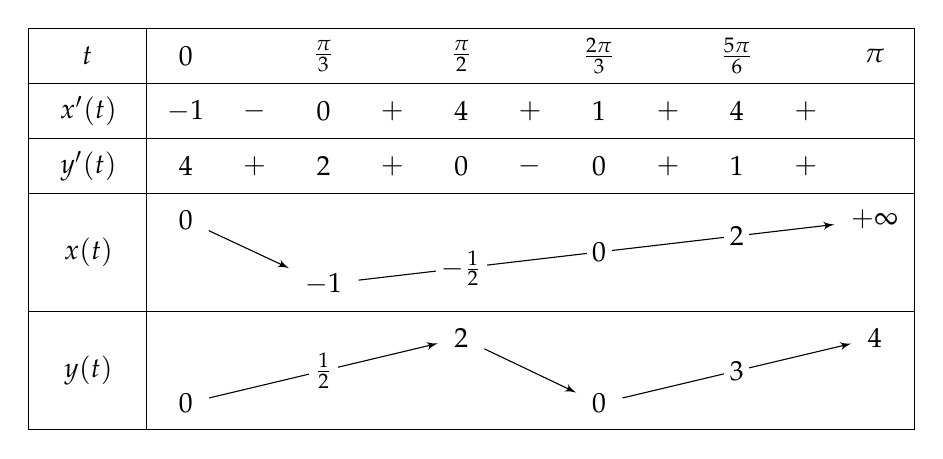
\begin{tikzpicture}
\tkzTabInit[lgt=1.5,espcl=1.75,deltacl=0.5]{$t$/0.7,$x'(t)$/0.7,$y'(t)$/0.7,$x(t)$/1.5,$y(t)$/1.5}{$0$,$\frac\pi3$,$\frac\pi2$,$\frac{2\pi}3$,$\frac{5\pi}6$,$\pi$}
\tkzTabLine{-1,-,0,+,4,+,1,+,4,+,}
\tkzTabLine{4,+,2,+,0,-,0,+,1,+,}
\tkzTabVar{+/$0$,-/$-1$,R/,R/,R/,+/$+\infty$}
\tkzTabIma{2}{6}{3}{$-\frac12$}
\tkzTabIma{2}{6}{4}{$0$}
\tkzTabIma{2}{6}{5}{$2$}
\tkzTabVar{-/$0$,R/,+/$2$,-/$0$,R/,+/$4$}
\tkzTabIma{1}{3}{2}{$\frac12$}
\tkzTabIma{4}{6}{5}{$3$}
\end{tikzpicture}
\end{center}
\begin{enumerate}
\item Dessiner, à partir du tableau, la courbe paramétrée par $f$.
\item Donner l'équation cartésienne de la tangente à la courbe au point de paramètre $t=\frac{5\pi}6$.
\item L'application $g=f_{|]0,\pi]}$ sera-t-elle injective ?
\item Quelle sera l'allure de la courbe entière si, pour $t\in[-\pi,\pi]$, (i) $f$ est impaire ? (ii) $f$ est
      $\pi$-périodique ?
\end{enumerate}
\place
\exercice{12}{3}{Ellipse et échelle}{Livre, exercice 2.2 · TD 2 de la classe}{lieu géométrique, tangence, déterminant}{td-c2}{6}
Une échelle tombe le long d'un mur. On note $\theta\in\left[0,\frac\pi2\right]$ l'angle entre l'échelle et l'horizontale. Soit $M$
un barreau de l'échelle.
\begin{enumerate}
\item Prouver que, dans un repère adapté, la courbe $\mathcal C$ parcourue par $M$ a pour représentation paramétrique
      $x(\theta)=a\cos\theta$, $y(\theta)=b\sin\theta$.
\item En déduire un dessin de $\mathcal C$ point par point en prenant $a=2$ et $b=1$.
\item À quel moment l'échelle est-elle tangente à la courbe $\mathcal C$ ?
\end{enumerate}
\place
\exercice{13}{2}{Symétries d'une courbe de Lissajous}{Exercice complémentaire}{symétries, réduction de l'intervalle}{c-sym}{7}
On pose $f(t)=(\sin2t,\ \sin3t)$. Montrer qu'on peut réduire l'étude à $\left[0,\frac\pi2\right]$ et expliquer comment obtenir la courbe entière.
\place
\exercice{14}{3}{Points d'inflexion}{Livre, exercice 2.4 · TD 6 de la classe}{inflexion, $\det(f',f'')$, branches paraboliques}{td-c6}{7}
On considère la courbe $\mathcal C$ définie pour $t\in\R$ par $x(t)=\frac14(t-2)^3$ et $y(t)=t^2-4$.
\begin{enumerate}
\item Étudier la courbe $\mathcal C$ sur $\R$. $\mathcal C$ admet-elle des asymptotes ?
\item Prouver que $\mathcal C$ possède exactement deux points d'inflexion.
\item Tracer $\mathcal C$ avec ses points d'inflexion.
\end{enumerate}
\place
\exercice{15}{2}{Position par rapport à une tangente}{Exercice complémentaire}{tangente, position globale, factorisation}{c-pos}{8}
On considère $f(t)=(t^2,t^3)$.
\begin{enumerate}
\item Donner l'équation de la tangente $T$ en $M(1)$.
\item Étudier la position de la courbe par rapport à $T$ et déterminer l'autre point d'intersection.
\end{enumerate}
\place
\exercice{16}{4}{Cardioïde}{Livre, exercice 2.3 · TD 4 de la classe}{angle moitié, point stationnaire, symétrie}{td-c4}{8}
On considère la courbe définie par $x(t)=(1-\cos t)\cos t$, $y(t)=(1-\cos t)\sin t$.
\begin{enumerate}
\item Donner son intervalle d'étude en repérant un axe de symétrie.
\item Prouver que $\cos t-\cos2t=\mathrm{Re}\big(e^{it}-e^{2it}\big)=2\sin\frac t2\sin\frac{3t}2$.
\item Donner le tableau de variation de $x$ et de $y$.
\item Donner la nature du point $O$ et la direction de sa tangente.
\item En déduire l'étude complète de la courbe $\mathcal C$.
\end{enumerate}
\place
\exercice{17}{4}{Lemniscate de Bernoulli}{Livre, exercice 2.7 · TD 5 de la classe}{symétrie $t\mapsto\frac1t$, point double, coordonnées polaires}{td-c5}{9}
Soit la courbe $\mathcal L$ parcourue par $M_t$ de coordonnées $x(t)=\dfrac t{1+t^4}$, $y(t)=\dfrac{t^3}{1+t^4}$. Faire l'étude de
$\mathcal L$ et prouver que la droite $y=x$ est axe de symétrie de la courbe. Vérifier que $\mathcal L$ a pour équation en
coordonnées polaires $r^2=\frac{\sin(2\theta)}2$ (\HP).
\place
\exercice{18}{4}{Cubique de Descartes}{Livre, exercice 2.8 · TD 8 de la classe}{asymptote oblique, position, symétrie $t\mapsto\frac1t$}{td-c8}{10}
On considère la courbe $\mathcal C$ : $x(t)=\dfrac t{1+t^3}$, $y(t)=\dfrac{t^2}{1+t^3}$.
\begin{enumerate}
\item Prouver que $M(t)$ et $M(1/t)$ sont symétriques par rapport à un axe $\Delta$.
\item Faire l'étude de la courbe pour $t\in\,]-1,1[$.
\item Prouver que, pour $t\to-1$, la courbe a pour asymptote $\mathcal D:y=-x-\frac13$ et déterminer la position de la courbe
      par rapport à $\mathcal D$.
\end{enumerate}
\place
\exercice{19}{3}{Étude complète avec point double}{Exercice complémentaire}{symétrie, variations, point double, branche parabolique, concavité}{c-tschirn}{11}
On considère la courbe $x(t)=t^2$, $y(t)=t^3-3t$, $t\in\R$.
\begin{enumerate}
\item Montrer que la courbe est symétrique par rapport à $(Ox)$.
\item Dresser le tableau de variations sur $\R_+$ ; préciser les tangentes horizontales et verticales.
\item Montrer que la courbe a un point double et donner l'angle de ses deux tangentes en ce point.
\item Étudier la branche infinie. La courbe a-t-elle des points d'inflexion ?
\item Tracer la courbe.
\end{enumerate}
\place
\exercice{20}{3}{La cycloïde}{Exercice complémentaire}{symétries, angle moitié, point stationnaire, tangente et normale}{c-cycloide}{11}
Un cercle de rayon $1$ roule sans glisser sur l'axe $(Ox)$ ; un point $M$ du cercle, initialement en $O$, décrit la cycloïde
\[f(t)=(t-\sin t,\ 1-\cos t),\qquad t\in\R,\]
où $t$ est l'angle dont le cercle a tourné ; le centre du cercle est alors $\Omega(t)=(t,1)$.
\begin{enumerate}
\item Comparer $f(t+2\pi)$ et $f(-t)$ à $f(t)$. En déduire un intervalle d'étude et la construction de la courbe entière.
\item Montrer que $f'(t)=2\sin\frac t2\left(\sin\frac t2,\ \cos\frac t2\right)$. Étudier les variations sur $[0,\pi]$ et déterminer les points stationnaires (on pourra utiliser l'exercice~\ref{e:c-cusp} pour leur nature).
\item Soient $H(t)=(t,2)$ et $K(t)=(t,0)$ le point le plus haut et le point de contact du cercle. Montrer que, en un point régulier, la tangente en $M(t)$ passe par $H(t)$ et la normale par $K(t)$.
\end{enumerate}
\place
\exercice{21}{3}{La développante du cercle}{Exercice complémentaire}{tangente, normale, point stationnaire, inflexion}{c-develop}{12}
On considère $f(t)=(\cos t+t\sin t,\ \sin t-t\cos t)$, $t\geq0$, et $P(t)=(\cos t,\sin t)$ sur le cercle unité $\mathcal C$.
\begin{enumerate}
\item Calculer $f'(t)$. Quels sont les points stationnaires ?
\item Montrer que $\vv{P(t)M(t)}=t\,(\sin t,\ -\cos t)$. En déduire que la droite $(PM)$ est tangente à $\mathcal C$ en $P$ et que $PM$ est égal à la longueur de l'arc de $\mathcal C$ allant de $(1,0)$ à $P$ (« fil que l'on déroule »).
\item Montrer que la normale à la courbe en $M(t)$ ($t>0$) est la droite $(PM)$.
\item Étudier le point $M(0)$ par un développement limité. La courbe a-t-elle des points d'inflexion ?
\end{enumerate}
\place
\clearpage
\partie{III}{Exercices de synthèse et approfondissement}{Courbes classiques étudiées en entier, rebroussements de seconde espèce, branches infinies délicates.}
\exercice{22}{4}{Cissoïde de Dioclès}{Livre, exercice 2.6 · TD 3 de la classe}{rebroussement, asymptote, lieu géométrique}{td-c3}{12}
Soit $a>0$ et la cissoïde $\mathcal C$ : $x(\theta)=2a\dfrac{\sin^3\theta}{\cos\theta}$, $y(\theta)=2a\sin^2\theta$.
\begin{enumerate}
\item Prouver que $\mathcal C$ possède un axe de symétrie. En déduire un intervalle d'étude.
\item Donner l'équation cartésienne de la tangente $T$ à $\mathcal C$ en $\theta=\frac\pi4$.
\item Donner les tableaux de variation de $x$ et $y$ en fonction de $\theta$.
\item Étudier les points stationnaires de $\mathcal C$.
\item Prouver que la cissoïde possède une asymptote $\mathcal D$ et donner la position de la courbe par rapport à son asymptote.
\item Construction point par point. Soit $A$ le projeté orthogonal de $O$ sur $\mathcal D$. On trace le cercle de diamètre
      $[OA]$ ; pour un point $Q$ du cercle, la droite $(OQ)$ coupe $\mathcal D$ en $H$, et l'on définit $P$ par $\vv{OP}=\vv{QH}$.
      Prouver que l'ensemble de ces points $P$ forme la cissoïde.
\end{enumerate}
\place
\exercice{23}{4}{Asymptote et prolongement}{Livre, exercice 2.10 · TD 10 de la classe}{asymptote, point limite, développement asymptotique}{td-c10}{13}
On considère la courbe paramétrée $\mathcal C$ par $x(t)=\frac1t$, $y(t)=\frac1{e^t-1}$.
\begin{enumerate}
\item Déterminer l'asymptote $\mathcal D$ à la courbe pour $t\to0$ et indiquer la position de la courbe par rapport à
      l'asymptote.
\item Vérifier que, pour $t\to+\infty$, la courbe $\mathcal C$ se prolonge en un point $A$. Déterminer la tangente à $\mathcal C$
      en ce point $A$.
\item Faire de même pour $t\to-\infty$.
\item En déduire ainsi le tracé de la courbe $\mathcal C$.
\end{enumerate}
\place
\exercice{24}{3}{L'astroïde}{Exercice complémentaire}{symétries, rebroussement, tangente}{c-astro}{14}
On considère $f(t)=(\cos^3t,\sin^3t)$, $t\in[0,2\pi]$.
\begin{enumerate}
\item Déterminer les symétries de la courbe et réduire l'intervalle d'étude.
\item Déterminer les points stationnaires et leur nature.
\item Donner l'équation de la tangente en un point régulier $M(t)$. Elle coupe les axes en $P$ et $Q$ : calculer $PQ$.
\end{enumerate}
\place
\exercice{25}{3}{La strophoïde}{Exercice complémentaire}{point double, tangentes, asymptote}{c-stroph}{15}
On considère $x(t)=\dfrac{t^2-1}{t^2+1}$, $y(t)=\dfrac{t(t^2-1)}{t^2+1}$, $t\in\R$.
\begin{enumerate}
\item Étudier les symétries.
\item Montrer que $O$ est un point double et que les tangentes en $O$ sont perpendiculaires.
\item Étudier les branches infinies et la position par rapport à l'asymptote.
\item Déterminer les tangentes horizontales et verticales, puis tracer la courbe.
\end{enumerate}
\place
\exercice{26}{5}{Bicorne : rebroussement de seconde espèce}{Livre, exercice 2.5 · TD 7 de la classe}{développement limité d'ordre 5, théorème $(p,q)$}{td-c7}{16}
Soit $\mathcal B$ représentée par $x(t)=\sin t$, $y(t)=\cos^5t+\frac12\cos^2t$.
\begin{enumerate}
\item Montrer que $M\left(\frac\pi2\right)$ est un point de rebroussement de seconde espèce.
\item Faire l'étude de la courbe en utilisant $\alpha=\arccos\left(\sqrt[3]{-\frac15}\right)$.
\item Dessiner la courbe, sachant qu'au point $A\in\mathcal B$, $A\simeq(0{,}8\,;0{,}1)$, la tangente est horizontale.
\end{enumerate}
\place
\exercice{27}{5}{Axe de symétrie oblique, parabole asymptote\HP}{Livre, exercice 2.9 · TD 9 de la classe}{symétrie $y=x$, point stationnaire, courbe asymptote}{td-c9}{17}
On considère la courbe $\mathcal C$ définie pour $t\in\R^*$ par $x(t)=t+\dfrac1{2t^2}$ et $y(t)=\dfrac{t^2}2+\dfrac1t$.
\begin{enumerate}
\item Prouver par DL que la courbe présente un point de rebroussement en $M(1)$, et dessiner la courbe au voisinage de
      $M(1)$.
\item Étudier $\mathcal C$ sur $\R^*$.
\item Prouver que $\mathcal C$ admet une parabole asymptote pour $t\to\pm\infty$.
\item Montrer que la droite $y=x$ est axe de symétrie orthogonale de $\mathcal C$. Quel sera le symétrique de $M(t)$ ?
\end{enumerate}
\place
\exercice{28}{4}{Le limaçon de Pascal}{Exercice complémentaire}{symétrie, variations, point double, inflexion}{c-limacon}{18}
On considère $f(t)=\big((1+2\cos t)\cos t,\ (1+2\cos t)\sin t\big)$, $t\in\R$.
\begin{enumerate}
\item Réduire l'intervalle d'étude à $[0,\pi]$.
\item Montrer que $x'(t)=-\sin t\,(1+4\cos t)$ et $y'(t)=4\cos^2t+\cos t-2$. Dresser le tableau de variations conjoint sur $[0,\pi]$ ; préciser les tangentes horizontales et verticales.
\item Montrer que $O$ est un point double et déterminer l'angle des deux tangentes en $O$.
\item Montrer que $\det(f',f'')=3(3+2\cos t)$. Conclure sur les points d'inflexion, puis tracer la courbe.
\end{enumerate}
\place
\exercice{29}{4}{Une courbe de Lissajous : synthèse}{Livre, exemple 2.9}{symétries, point double, intersection avec une droite, inflexion}{ex-liss}{18}
On considère $f(t)=(\cos3t,\ 2\sin t)$, $t\in\R$.
\begin{enumerate}
\item Réduire l'intervalle d'étude, puis étudier la courbe et la tracer.
\item Montrer que $J=(0,1)$ est un point double et donner les équations des tangentes $T_1$ et $T_2$ en $J$.
\item Déterminer les autres points communs à la courbe et à la tangente $T_2:y=\frac x{\sqrt3}+1$.
\item Déterminer les points d'inflexion.
\end{enumerate}
\place
\clearpage
\partie{IV}{Exercices difficiles et type concours}{Études complètes, sans indication de méthode, dans l'esprit des épreuves écrites.}
\exercice{30}{5}{Problème type devoir surveillé}{Livre, exercice 2.11 · problème type devoir}{étude complète, point stationnaire, position globale, asymptotes, inflexion}{ds-pb}{20}
On considère la courbe $\mathcal C$ définie par
\[x(t)=\frac4t+\ln(3+t),\qquad y(t)=t+\frac4t,\qquad t\in\,]-3,0[\,\cup\,]0,+\infty[,\]
et l'on note $M(t)$ le point de paramètre $t$, $f(t)=\vv{OM(t)}$. Valeurs utiles : $\ln3\approx1{,}10$,
$\ln5\approx1{,}61$, $\ln9\approx2{,}20$, $\ln15\approx2{,}71$.
\begin{enumerate}
\item \textbf{Étude générale et points remarquables.}
\begin{enumerate}
\item Factoriser $x'(t)$ et $y'(t)$, puis dresser le tableau de variations conjoint de $x$ et $y$.
\item Déterminer le point $A$ où la tangente est verticale et le point $B$ où elle est horizontale.
\item Montrer que, en un point régulier, la pente de la tangente vaut $p(t)=\frac{(t-2)(t+3)}{t-6}$. Pour quelles valeurs
      de $m$ existe-t-il un point où la tangente a pour pente $m$ ? Montrer qu'il existe un unique point $H$ où cette pente
      vaut $25$.
\end{enumerate}
\item \textbf{Étude du point $C=M(-2)$.}
\begin{enumerate}
\item En posant $t=-2+h$, écrire le développement limité de $f$ à l'ordre $3$ en $-2$.
\item En déduire la nature du point $C$ et montrer que la tangente $T_C$ a pour équation $x-2y=6$.
\item Préciser la position \emph{locale} de $\mathcal C$ par rapport à $T_C$.
\item En étudiant $\varphi(t)=x(t)-2y(t)-6$, déterminer la position \emph{globale} de $\mathcal C$ par rapport à $T_C$.
\end{enumerate}
\item \textbf{Asymptotes.}
\begin{enumerate}
\item Montrer que $\mathcal C$ admet une asymptote $\Delta_0$ lorsque $t\to0$ et préciser la position.
\item Montrer que $\mathcal C$ admet une autre asymptote $\Delta'$ lorsque $t\to-3$ et préciser la position.
\end{enumerate}
\item \textbf{Branche $t\to+\infty$ (\HP).}
\begin{enumerate}
\item Quelle est la nature de cette branche ?
\item Soit $\mathcal E:y=e^x-7$. En utilisant le point de $\mathcal E$ de même abscisse que $M(t)$, montrer que $\mathcal E$
      est asymptote à $\mathcal C$, et préciser la position.
\item Montrer qu'en utilisant le point de même \emph{ordonnée}, on prouverait de même que toute courbe $y=e^x+c$ est
      asymptote à $\mathcal C$. Commenter.
\end{enumerate}
\item \textbf{Point d'inflexion.}
\begin{enumerate}
\item Écrire $f'(t)=\lambda(t)\,\ve g(t)$ avec $\lambda(t)=\frac{t+2}{t^2(t+3)}$ et $\ve g(t)$ à coordonnées polynomiales,
      puis montrer que $\det\big(f'(t),f''(t)\big)=\lambda(t)^2\det\big(\ve g(t),\ve g'(t)\big)$.
\item En déduire que $\mathcal C$ possède un unique point d'inflexion $N$. Le comparer à $H$ et expliquer.
\item Donner une équation de la tangente $T_N$.
\end{enumerate}
\item \textbf{Dessin.} Tracer $\mathcal C$ en plaçant $A$, $B$, $C$, $N$, les tangentes en ces points et les asymptotes.
\end{enumerate}
\place
\exercice{31}{5}{Étude complète d'une courbe rationnelle (type concours)}{Exercice complémentaire}{symétrie, rebroussement, asymptotes, concavité}{c-concours}{22}
On considère la courbe $\mathcal C$ définie par $x(t)=\dfrac{t^2}{t-1}$, $y(t)=\dfrac{t^2}{t+1}$, $t\in\R\setminus\{-1,1\}$.
\begin{enumerate}
\item Comparer $M(-t)$ et $M(t)$. En déduire une symétrie de $\mathcal C$ et un intervalle d'étude.
\item Factoriser $x'(t)$ et $y'(t)$ ; dresser le tableau de variations conjoint sur $[0,1[\,\cup\,]1,+\infty[$.
\item Étudier le point $M(0)$ : nature et tangente.
\item Étudier les branches infinies ; préciser la position de $\mathcal C$ par rapport à ses asymptotes.
\item Calculer $\det(f',f'')$. La courbe a-t-elle des points d'inflexion ?
\item Tracer $\mathcal C$ avec ses asymptotes et ses tangentes remarquables.
\end{enumerate}
\place
\exercice{32}{5}{Une cubique à rebroussement (type concours)}{Exercice complémentaire}{équation cartésienne, rebroussement, asymptote, inflexion}{c-concours2}{23}
On considère la courbe $\mathcal C$ définie par $x(t)=\dfrac{t^2}{1+t}$, $y(t)=\dfrac{t^3}{1+t}$, $t\in\R\setminus\{-1\}$.
\begin{enumerate}
\item Montrer que $\mathcal C$ est contenue dans la courbe d'équation $x^2(x+y)=y^2$.
\item Factoriser $x'(t)$ et $y'(t)$ et dresser le tableau de variations conjoint. Préciser les tangentes horizontales et verticales.
\item Étudier le point $M(0)$.
\item Étudier les branches infinies et la position de $\mathcal C$ par rapport à son asymptote.
\item Calculer $\det(f',f'')$ et déterminer les points d'inflexion.
\item Tracer $\mathcal C$.
\end{enumerate}
\place
\end{document}
